\section{Backend des Web-Editors}\label{sec:editor-backend}
Das Backend des Web-Editors basiert auf einem mit Spring Initializr generiertem Java Projekt.
Zusätzlich wurden bei der Konfiguration die Dependencies für eine Spring Web Anwendung hinzugefügt.
Neben den eben genannten Dependencies wurde lediglich fulibWorkflows als weitere Bibliothek zum Backend hinzugefügt.

Die verfügbaren Endpunkte des Backends werden in einem Controller bereitgestellt.
In diesem Fall ist dies der FulibWorkflowsController, welcher mit zwei Annotations versehen ist.
Die erste Annotation ist~\texttt{@Controller}, welche der Anwendung mitteilt, dass diese Klasse als Controller agiert.
Bei der zweiten Annotation handelt es sich, um \texttt{@CrossOrigin()} mit welcher es ermöglicht wird, problemlos mit dem
Frontend zu interagieren.
Im FulibWorkflowsController sind Endpunkte für die Generierung und den Download definiert.
Diese Definitionen werden in Listing~\ref{listing:endpoints} zur Veranschaulichung dargestellt.

\begin{listing}[!ht]
    \inputminted[firstnumber=15]{java}{listings/3.3/Endpoints.java}
    \caption{Definition der Endpunkte}
    \label{listing:endpoints}
\end{listing}

Beide Endpunkte können mit einem POST-Request angesprochen werden, da sowohl beim Download als auch der Generierung der Inhalt der
yaml Datei vom Frontend mitgeschickt wird.
Dies sorgt dafür, dass bei beiden Endpunkten die Generierung durchgeführt wird, um kein Abspeichern von Dateien und Vergabe von IDs für
eine Beschreibung angelegt und verwaltet werden muss.
Damit die Endpunkte auf diesen Inhalt zugreifen können, ist der erste Methodenparameter mit der \texttt{@RequestBody} Annotation versehen.
Hierbei wird auf den Inhalt zugegriffen, welcher vom Frontend in der Post-Anfrage mitgesendet wurde.
Der Downlaod-Endpunkt erhält zusätzlich zu der yaml Beschreibung ebenfalls Query-Parameter.
Diese enthalten die aus dem Download-PopUp des Frontends angegeben Dateien, welche heruntergeladen werden sollen.
Mittels der \texttt{@ResponseBody} Annotation, können der Antwort des Backends weitere Daten hinzugefügt werden, in welcher Form diese
sind, resultiert aus dem Rückgabetyp der jeweiligen Methode unterhalb der Annotation.
Bei der Generate-Methode wird ein JSON-Objekt als String zurückgegeben, wobei bei der Download-Methode das generierte Zip-Archiv als ByteArray verwendet wird.
Beide Methoden des Controllers reichen die erhaltenen Daten an den FulibWorkflowsService weiter, welcher sich um die Generierung über fulibWorkflows
und der Erstellung des Zip-Archives kümmert.

Im FulibWorkflowsService, wird sowohl in der generate- als auch der createZip-Methode, welche vom Controller aufgerufen werden,
der yaml-String über fulibWorkflows generiert.
Dabei nutzt das Backend die \texttt{generateAndReturnHTMLsFromString}-Methode des BoardGenerators von fulibWorkflows.
Im Anschluss wird aus der Map von generierten Dateien ein GenerateResult erstellt, welches von der generate-Methode zu einem JSON-String weiterverarbeitet und zurück an den Controller gibt.
Nachdem das GenerateResult-Objekt in der createZip-Methode erstellt wurde, beginnt das Erstellen des Zip-Archivs.
Auf Grundlage der Query-Parameter werden lediglich die Dateien zum Zip-Archiv hinzugefügt, welche im Frontend ausgewählt werden.
In Abbildung~\ref{fig:export} sollen alle Dateien heruntergeladen werden, welche von fulibWorkflows generiert wurden.

\begin{figure}[h]
    \centering
    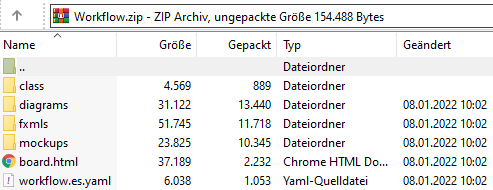
\includegraphics[width=0.6\textwidth]{images/3.3/export}
    \caption{Inhalt eines heruntergeladenen Zip-Archivs}
    \label{fig:export}
\end{figure}

Um die Dateien strukturiert zu halten, werden Diagramme und Mockups in eigenen Unterordner abgelegt.
Hierbei wird zwischen Objektdiagrammen und dem Klassendiagramm, als auch zwischen HTML- und FXML-Mockups unterschieden.
Auf oberster Ebene werden sowohl die Workflow-Beschreibung als auch das generierte Event Storming Board abgelegt, da diese
die Grundlage für alle weiteren Dateien legen.
Das Klassendiagramm ist im Ordner \textit{class} abgelegt, die Objektdiagramme im \textit{diagrams}-Ordner.
Im Gegensatz hierzu, werden die HTML-Mockups im \textit{mockups}-Ordner hinterlegt, die gleichen Mockups im FXML-Format werden
im \textit{fxmls}-Ordner platziert.
